\documentclass[11pt,border=5pt]{standalone}
\usepackage{fontspec}
\setmainfont{cmunrm.otf}[BoldFont=cmunbx.otf,ItalicFont=cmunti.otf,BoldItalicFont=cmunbi.otf]
\usepackage{amsmath}
\usepackage{unicode-math}
\setmathfont{NewCMMath-Regular.otf}
\usepackage{tikz}
\usetikzlibrary{arrows.meta,patterns,angles,quotes}
\begin{document}
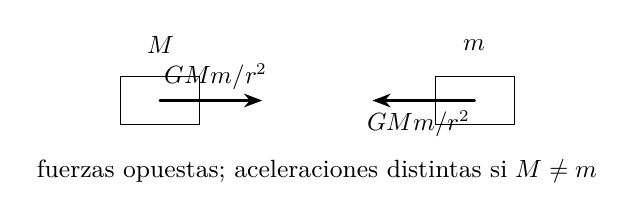
\begin{tikzpicture}[>=Stealth,font=\small,line cap=round,line join=round]
\draw[fill=white] (-2.5,-0.3) rectangle (-1.5,0.3);
\node at (-2,0) {};
\draw[fill=white] (1.5,-0.3) rectangle (2.5,0.3);
\node at (2,0) {};
\node at (-2,0.7) {$M$};
\node at (2,0.7) {$m$};
\draw[->,thick] (-2,0) -- (-0.7,0) node[pos=0.55,above] {$G Mm/r^2$};
\draw[->,thick] (2,0) -- (0.7,0) node[pos=0.55,below] {$G Mm/r^2$};
\node at (0,-0.9) {fuerzas opuestas; aceleraciones distintas si $M\ne m$};

\end{tikzpicture}
\end{document}
